\def\patch{\omega _j}
\subsection{$\mathcal{T}^{\Omega}_h$ non conforming to $\Gamma$ and $\Lambda$} \label{sec:unfit2}
We analyze now the case in which the elements of the 3D mesh $\mathcal{T}^{\Omega}_h$ do not conform with the surface $\Gamma$ nor with $\Lambda$. In this case, the 3D-1D-1D
formulation, namely Problem 2, is more suitable. 
%{\color{red} Add more details, we can refer also to cutFEM (Burman, Massing etc.) explaining the limitation of that approach (network case for example).}\\
Therefore we focus on the analysis of this discretization approach for Problem 2 solely.

\subsubsection{Problem 2} We consider for the solutions $u_h$ and ${\ud}_h$ the spaces $X_h = X_{h,0}^1(\Omega) \times X_{h^\prime,0}^1(\Lambda)$. With little abuse of notation, we assume that the characteristic mesh size of the 3D mesh $\mathcal{T}^{\Omega}_h$ and the one of the 1D mesh $\mathcal{T}^{\Lambda}_{h'}$ are different. Concerning the multiplier space, let $\mathcal{G}_h = \{K \in \mathcal{T}^{\Omega}_h: \, K\cap \Lambda \neq \emptyset\}$, be the set of the 3D elements that intersect $\Lambda$. Then we define $Q_h=\{{\ld}_h : {\ld}_h \in P^0(K) \, \forall K \in \mathcal{G}_h\}$. We notice that the multiplier functions are defined on the 3D elements. With little abuse of notation, we denote with $Q_h$ also the restriction to $\Lambda$ of the space of piecewise constant functions defined in 3D. As a result, we have $Q_h \subset L^2(\Lambda) \subset H^{-\frac12}(\Lambda)$.
With this choice of multipliers the problem is not inf-sup stable, therefore the idea is to add a stabilization term $s({\ld}_h, {\md}_h): \ Q_h \times Q_h \rightarrow \mathbb{R}$ to \eqref{eq:prob2_discrete} following the approach introduced in \cite{burman2014}. 
The objective of this section is to analyze the stabilized version of the 3D-1D-1D problem: find $[u_h, {\ud}_h] \in X_h$ and ${\ld}_h \in Q_h$ such that
\begin{multline}\label{eq:prob2_stabilized}
a([u_h, {\ud}_h], [v_h, {\vd}_h]) +
b([v_h, {\vd}_h], {\ld}_h)
+ b([u_h, {\ud}_h], {\md}_h)
- s({\ld}_h, {\md}_h) 
= c(v_h) + d({\md}_h)\\
  \quad \forall [v_h, {\vd}_h] \in X_h, \,
  \forall {\md}_h \in Q_h\,.
\end{multline}
The idea of the stabilization strategy proposed in \cite{burman2014}
is to identify a new multiplier space $Q_H$, which is never implemented in practice, such that inf-sup stability with $X_h$ holds true. Then, the stabilization operator is designed to control the distance between $Q_h$ and $Q_H$ trough the following inequality
\begin{equation*}
    \|{\md}_h - \pi_H {\md}_h\|_{Q_H} \leq C s_h({\md}_h, {\md}_h)\,,
\end{equation*}
being $\pi_H$ a suitable projection operator $Q_h \rightarrow Q_H$. Applying the results obtained in \cite{burman2014} we will show that the well posedness of problem \eqref{eq:prob2_stabilized} is governed by the following lemma.
\begin{lemma}[Lemma 2.3 of \cite{burman2014}]\label{lemma23burman}
\begin{enumerate}
    \item If the $b(\cdot,\cdot),\, X_h,Q_H \rightarrow \R$ is inf-sup stable.
    \item If the stabilization operator $s_h(\cdot,\cdot),\, Q_H,Q_H \rightarrow \R$ is such that
    \begin{equation*}
        \beta \|{\md}_h\|_{H^{-\frac12}(\Lambda)} \leq \sup\limits_{v_h \in X_h} \frac{b(v_h,{\md}_h}{\vertiii{v_h})} + s_h({\md}_h, {\md}_h), \quad \forall {\md}_h \in Q_h\,.
    \end{equation*}
    \item If for any $[v_h, {\vd}_h]$ there exists a function $\xi_h\in Q_h$ depending on $[v_h, {\vd}_h]$, namely $\xi_h=\xi_h([v_h, {\vd}_h])$, s.t.
\begin{gather}
\label{stab_coercivity}
a([v_h, {\vd}_h],[v_h, {\vd}_h] ) + b([v_h, {\vd}_h], \xi_h) \geq \alpha_\xi \vertiii{[v_h, {\vd}_h]}_{X_h}\,,
\\
\label{stab_stability}
(s(\xi_{h}, \xi_{h}))^{\frac 12} \leq c_s \vertiii{[v_h, {\vd}_h]}_{X_h}\,,
\end{gather}
being $\vertiii{[\cdot \, ,\, \cdot] }_{X_h}$ a suitable discrete norm. 
\end{enumerate}
Then, problem \eqref{eq:prob2_stabilized} admits a unique solution.
\end{lemma}
For the proof of this result we remand the reader to Lemma 2.3 of \cite{burman2014}. In the reminder of this section we show how to find a multiplier space $Q_H$ and a stabilization operator $s_h$ such that all the assumptions of lemma \ref{lemma23burman} are satisfied.

% The stabilization operator is based on a new multiplier space $Q_H$, for which the discrete inf-sup condition is fulfilled, and a projection operator $\pi_H: Q_h \rightarrow Q_H$ such that for any $[v, \vd] \in X $
% \begin{equation}\label{condition_pi_L}
% b([v, \vd], {\ld}_h - \pi_H {\ld}_h) \leq C \vertiii{[v,\vd]}\|{\ld}_h - \pi_H {\ld}_h\|_{Q_H},
% \end{equation}
% where for $X$ and $\vertiii{[\cdot, \cdot]}$ we use the definitions of section $3.2$ and $\|\cdot \|_{Q_H}$ denotes a suitable discrete norm on $Q_H$. Then, the following relaxed form of the inf-sup condition is satisfied,
% \begin{lemma}\cite[Lemma2.1]{burman2014}\label{lemma_burman2014}
% If the multiplier space $Q_H$ is inf-sup stable and the operator $\pi_H: Q_h \rightarrow Q_H$ satisfies \eqref{condition_pi_L}, then for any ${\ld}_h \in Q_h$ it holds,
% \begin{equation*}
% \|{\ld}_h\|_{H^{-\frac 12}(\Lambda)} \lesssim \sup_{\substack{v_h \in X_{h,0}^1(\Omega)\\ {\vd}_h \in X_{h^\prime,0}^1(\Lambda)}} \frac{b([v_h, {\vd}_h], {\ld}_h)}{\vertiii{[v_h, {\vd}_h]}} + \|{\ld}_h - \pi_H {\ld}_h\|_{Q_H}.
% \end{equation*}
% \end{lemma}
%  Based on this projection operator, we build the stabilization term $s({\ld}_h, {\md}_h)$ satisfying
%  \begin{equation}\label{condition_pi_L_bis}
%  \|{\ld}_h- \pi_H {\ld}_h\|_{Q_H} C \leq s({\ld}_h, {\ld}_h)
% \end{equation} and prove that for any $[u_h, {\ud}_h]$ there exists a function $\xi_h\in Q_h$ depending on $[u_h, {\ud}_h]$, namely $\xi_h=\xi_h([u_h, {\ud}_h])$, s.t.
% \begin{equation}\label{stab_coercivity}
% a([u_h, {\ud}_h],[u_h, {\ud}_h] ) + b([u_h, {\ud}_h], \xi_h) \geq \alpha_\xi \vertiii{[u_h, {\ud}_h]}_{X_{h,0}^1(\Omega)\times X_{h^\prime,0}^1(\Lambda) },
% \end{equation}
% \begin{equation}\label{stab_stability}
% (s(\xi_{h}, \xi_{h}))^{\frac 12} \leq c_s \vertiii{[u_h, {\ud}_h]}_{X_{h,0}^1(\Omega)\times X_{h^\prime,0}^1(\Lambda) },
% \end{equation}
% being $\vertiii{[\cdot \, ,\, \cdot] }_{X_{h,0}^1(\Omega)\times X_{h^\prime,0}^1(\Lambda) }$ a suitable discrete norm. 


The first step consists of showing
that there exists a discrete space $Q_H$ that satisfies the first assumption of \ref{lemma23burman}. 
We recall that in the case of Problem 2, 
\begin{equation*}
b([u_h, {\vd}_h], {\md}_h) = \left(\mtrace v_h - {\vd}_h, {\md}_h\right)_{\Lambda,|\DD|}.
\end{equation*}
The construction of the inf-sup stable space $Q_H$ is based on macro elements of diameter $H$, where $H$ is sufficiently large. In particular, we assume that there exists positive constants $c_h$ and $c_H$ such that $c_h h\leq H \leq c_H^{-1}h$, being $h$ the mesh characteristic size of $\mathcal{T}_h^\Omega$. The space is constructed assembling the 3D elements of $\mathcal{G}_h$ into macro patches $ \patch $ such that $H \leq |\patch\cap \Lambda|\leq cH$, with $c\geq 1$. Let $M_j$ be the number of elements of the patch $\omega_j$, namely, $\patch=\cup _{i=0}^{M_j} K_i$, where $K_i \in \mathcal{G}_h$, $M_j$ is uniformly bounded in $j$ by some $M\in \mathbb{N}$ and $H=\min_{j}|\patch\cap \Lambda|$. We assume that the interiors of the patches $\patch$ are  disjoint. We define 
\begin{equation*}
Q_H=\left\{{\md }_H: \, {\md }_H\in P^0(\patch)\, \forall j \right\}.
\end{equation*}
As previously pointed out for $Q_h$, we denote with $Q_H$ also the restriction of the multiplier space to $\Lambda$, namely say $Q_H \subset L^2(\Lambda) \subset H^{-\frac12}(\Lambda)$.

%figure extended patch
\begin{figure}\label{fig:patch}
\center
%\documentclass[tikz,border=3mm]{standalone}
%\begin{document}

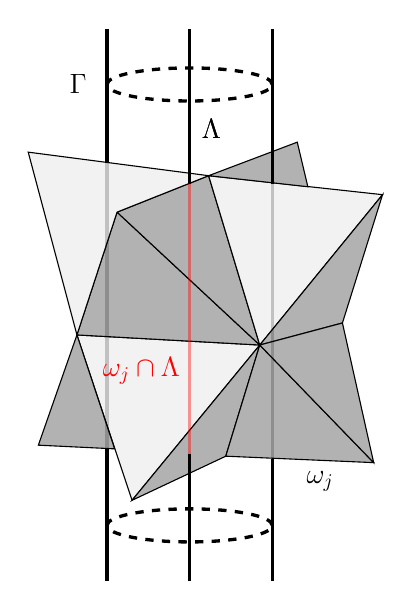
\begin{tikzpicture}[scale=0.7, every node/.style={scale=0.7}]
\pgfmathsetmacro{\factor}{1/sqrt(2)};
\coordinate  (A) at (2,0,-1*\factor);
\coordinate  (B) at (2.2,-1.2,2*\factor);
\coordinate  (C) at (-0.5,1,2*\factor);
\coordinate  (D) at (0.5,-2,2*\factor);
\coordinate  (E) at (0.5,3.5,3*\factor);
\coordinate  (F) at (0.8,2.8,-2*\factor);
\coordinate  (G) at (-1.2,-1,2*\factor);
\coordinate  (H) at (5.7,-0.5,5*\factor);
\coordinate  (I) at (1,-0.25,5*\factor);
\coordinate  (L) at (-2.5,3.2,-2.1*\factor);
\coordinate  (M) at (4.5,3,0*\factor);
\coordinate  (N) at (3.5,0.4,-1*\factor);
\coordinate  (O) at (2,3,-3.5*\factor);
\coordinate  (P) at (2.6,2.6,-2*\factor);
%\draw[->] (0,0) -- (3,0,0) node[right] {$x$};
%\draw[->] (0,0) -- (0,3,0) node[above] {$y$};
%\draw[->] (0,0) -- (0,0,3) node[below left] {$z$};
%\foreach \i in {A,B,C,D}
%\draw[dashed] (0,0)--(\i);
\draw[black, fill=white!90!gray] (A)--(D)--(C)--cycle;
\draw[black,  fill=gray!60!] (A) --(B)--(D)--cycle;
\draw[black, fill=gray!60!] (E) --(C)--(A)--cycle;
\draw[black,   fill=gray!60!] (E) --(F)--(A)--cycle;
\draw[black,    fill=gray!60!] (B) --(A)--(H)--cycle;
\draw[black,    fill=gray!60!] (C) --(G)--(I)--cycle;
\draw[black, fill=white!90!gray] (C) -- (E) -- (F)--(L)--cycle;
\draw[black,  fill=white!90!gray] (A) --(F)--(M)--cycle;
\draw[black,   fill=gray!60!] (A) --(N)--(M)--cycle;
\draw[black,    fill=gray!60!] (A) --(N)--(H)--cycle;
\draw[black,    fill=gray!60!] (F) --(O)--(P)--cycle;
%\draw[-, fill=gray!30!blue, opacity=.2] (E) --(G)--(H)--cycle;
\node [font=\Large, right] at (3, -2.2) {$\omega_j$};


%cylinder Gamma
\draw[dashed, very thick] (1, 5) ellipse (1.5 and 0.3);
\draw[dashed, very thick] (1, -3) ellipse (1.5 and 0.3);
\draw[black, very  thick] (-0.5, 3.6) -- (-0.5, 6);
\draw[black, very thick, opacity=.2] (-0.5, 3.6) -- (-0.5, -1.6);
\draw[black, very  thick] (-0.5, -1.6) -- (-0.5, -4); 
\draw[ very thick] (2.5, 6) -- (2.5, 3.2);
\draw[ very thick, opacity =0.2] (2.5, 3.2) -- (2.5, -1.8);
\draw[very thick] (2.5, -1.8) -- (2.5, -4);
\node [font=\Large, right] at (-1.3, 5) {$\Gamma$};

%centerline \Lambda
\draw[very thick] (1, 6) -- (1, 3.2);
\draw[red, very thick, opacity=.4] (1, 3.2) -- (1, -1.8);
\draw[very thick, ]  (1, -1.7) -- (1, -4);
\node [font=\Large, right] at (1.1, 4.2) {$\Lambda$};
\node [font=\Large, right] at (1.1, 4.2) {$\Lambda$};
\node [font=\Large, right, red] at (-0.7, -0.2) {$\omega _j \cap \Lambda$};
\end{tikzpicture}



%\end{document}
\caption{Extended patches $\omega_j$.}
\end{figure}

Moreover, we associate to each patch $\patch$ a shape-regular extended patch, still denoted by $\omega_j$ for notational simplicity, which is built adding to $\patch$ a sufficient number of elements of $\mathcal{T}_h^{\Omega}$ and we assume that the interiors of the new extended patches $\omega _j$ are still disjoint (see Figure \ref{fig:patch}). Here we are using the classical definition of shape-regularity, see for example \cite{MR2050138}, namely there exist a constant $C>0$ such that for any $\omega_j$, $\frac{\tilde{\rho}_j}{\bar{\rho}_j}\leq C$, being $\tilde{\rho}_j$ the diameter of $\omega_j$ and $\bar{\rho}_j$ the diameter of the largest ball that can be inscribed in $\omega_j$. The extended patches $\omega _j$ are built such that they fulfill the conditions meas$(\patch)=\mathcal{O}(H^3)$ and diam$(\Gamma_{\patch\cap \Lambda}\cap \omega_j)=\mathcal{O}(H)$, where $\Gamma_{\patch\cap \Lambda}$ is the portion of $\Gamma$ with centerline $\patch\cap \Lambda$. The latter assumption is required to ensure that the intersection of $\Gamma_{\patch\cap \Lambda}$ and $\omega_j$ is not too small and it will be needed later on to prove the inf-sup stability of the space $Q_H$ in Lemma \ref{lemma:Lh_infsup}. A representation of this construction in the simple case in which $\omega _j$ is composed just by one tetrahedron is shown in Figure \ref{fig:gamma_generated}.

% As shown in \cite[Section III]{burman2014}, we can always choose $\pi_H$ as the $L_2$ orthogonal projection operator from $\Lambda_h$ to $Q_H$ in order to satisfy \eqref{condition_pi_L} and then in practice replace it with any interpolation $\tilde{\pi}_L$ of $\Lambda_h$ in $Q_H$. In particular, for any $\lambda_h \in \Lambda_h$ we define,
% \begin{equation*}
% \tilde{\pi}_L {\ld}_{ _{|\patch}} = M_j^{-1} \sum_{\substack{i: \ K_i \in \mathcal{G}_h, \  K_i \cap \omega_j \neq \emptyset}} {\ld}_{|K_i} \qquad \text{for all $\omega_j$,} 
% \end{equation*}
% being $M_j$ the cardinality of the set $\{i: \ K_i \in \mathcal{G}_h, \  K_i \cap \omega_j \neq \emptyset\}$. These choices lead to the following stabilization 
% \begin{equation}\label{eq:stab}
% s({\ld}_h, {\md}_h)= \sum _{K\in \mathcal{G}_{h}} \int_{\partial K\setminus \partial \mathcal{G}_{h}} h \llbracket {\ld}_h \rrbracket \llbracket {\md}_h \rrbracket,
% \end{equation}
% being $\llbracket {\ld}_h \rrbracket$ the jump of ${\ld}_h$ across the internal faces of $\mathcal{G}_h$.

\begin{figure}\label{fig:gamma_generated}
\centering
\subfigure[$\Gamma_{\omega_j \cap \Lambda}$]
{
%\documentclass[tikz,border=3mm]{standalone}
%\usetikzlibrary{calc}
%\usetikzlibrary{shapes, snakes, patterns, arrows}
%\begin{document}

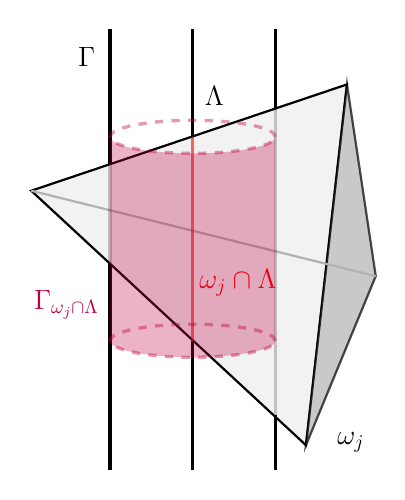
\begin{tikzpicture}[scale=0.7, every node/.style={scale=0.7}]
\pgfmathsetmacro{\factor}{1/sqrt(2)};


\coordinate  (A) at (-2.5,1.5,-2.1*\factor);
\coordinate  (B) at (3.8,4,0*\factor);
\coordinate  (C) at (3.6,-2,2*\factor);
\coordinate  (D) at (6.5,2.7,8*\factor);
\draw[thick, black,    fill=white!90!gray, opacity=1] (A) --(B)--(C)--cycle;
\draw[ thick,black,  fill=gray!60!, opacity=0.7] (D) --(B)--(C)--cycle;
\draw[thick,gray!60!] (D) --(A);
\node [font=\Large, right] at (3.5, -2.5) {$\omega_j $};


%cylinder Gamma
%\draw[dashed, very thick] (1, 5) ellipse (1.5 and 0.3);
%\draw[dashed, very thick] (1, -3) ellipse (1.5 and 0.3);
\draw[black, very  thick] (-0.5, 2.55) -- (-0.5, 5);
\draw[black, very thick, opacity=.2] (-0.5, 2.55) -- (-0.5, 0.75);
\draw[black, very  thick] (-0.5, 0.75) -- (-0.5, -3); 
\draw[ very thick] (2.5, 5) -- (2.5, 3.55);
\draw[ very thick, opacity =0.2] (2.5, 3.55) -- (2.5, -2);
\draw[very thick] (2.5, -2) -- (2.5, -3);
\node [font=\Large, right] at (-1.2, 4.5) {$\Gamma$};


%centerline \Lambda
\draw[very thick] (1, 5) -- (1, 3.05);
\draw[red, very thick, opacity=.6] (1, 3.05) -- (1, -0.65);
\draw[very thick, ]  (1, -0.65) -- (1, -3);
\node [font=\Large, right] at (1.1, 3.8) {$\Lambda$};
\node [font=\Large, right, red] at (1, 0.4) {$\omega _j \cap \Lambda$};

\draw[dashed, very thick, purple, opacity=.4] (1, 3.05) ellipse (1.5 and 0.3);
\draw[dashed, very thick, purple, opacity=.4] (1, -0.65) ellipse (1.5 and 0.3);

\fill [purple, opacity=0.3]  (-0.5, -0.65) arc (180:360:1.5 and 0.3) -- (2.5, 3.05) arc (0:180:1.5 and -0.3);
\node [font=\Large, right, purple] at (-2, 0) {$\Gamma_{\omega_j \cap \Lambda}$};

\end{tikzpicture}

%\end{document}
}
\qquad \qquad
\subfigure[ $\Gamma_{\omega_j \cap \Lambda} \cap \omega_j$]{
%\documentclass[tikz,border=3mm]{standalone}
%\usetikzlibrary{calc}
%\usetikzlibrary{shapes, snakes, patterns, arrows}
%\begin{document}
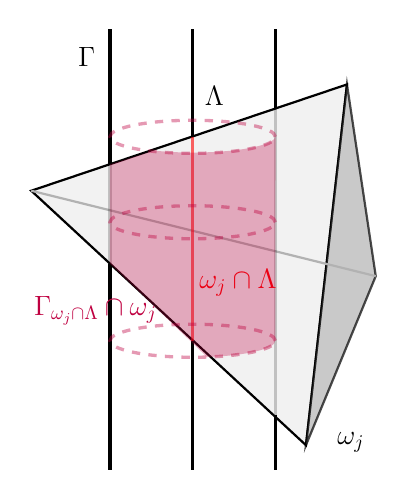
\begin{tikzpicture}[scale=0.7, every node/.style={scale=0.7}]

\pgfmathsetmacro{\factor}{1/sqrt(2)};

%tetrahedron
\coordinate  (A) at (-2.5,1.5,-2.1*\factor);
\coordinate  (B) at (3.8,4,0*\factor);
\coordinate  (C) at (3.6,-2,2*\factor);
\coordinate  (D) at (6.5,2.7,8*\factor);
\draw[thick, black,    fill=white!90!gray, opacity=1] (A) --(B)--(C)--cycle;
\draw[ thick,black,  fill=gray!60!, opacity=0.7] (D) --(B)--(C)--cycle;
\draw[thick,gray!60!] (D) --(A);
\node [font=\Large, right] at (3.5, -2.5) {$\omega_j $};


%cylinder Gamma
%\draw[dashed, very thick] (1, 5) ellipse (1.5 and 0.3);
%\draw[dashed, very thick] (1, -3) ellipse (1.5 and 0.3);
\draw[black, very  thick] (-0.5, 2.55) -- (-0.5, 5);
\draw[black, very thick, opacity=.2] (-0.5, 2.55) -- (-0.5, 0.75);
\draw[black, very  thick] (-0.5, 0.75) -- (-0.5, -3); 
\draw[ very thick] (2.5, 5) -- (2.5, 3.55);
\draw[ very thick, opacity =0.2] (2.5, 3.55) -- (2.5, -2);
\draw[very thick] (2.5, -2) -- (2.5, -3);
\node [font=\Large, right] at (-1.2, 4.5) {$\Gamma$};

%centerline \Lambda
\draw[very thick] (1, 5) -- (1, 3.05);
\draw[red, very thick, opacity=.6] (1, 3.05) -- (1, -0.65);
\draw[very thick, ]  (1, -0.65) -- (1, -3);
\node [font=\Large, right] at (1.1, 3.8) {$\Lambda$};
\node [font=\Large, right, red] at (1, 0.4) {$\omega _j \cap \Lambda$};

%intersection
\draw[dashed, very thick, purple, opacity=.4] (1, 3.05) ellipse (1.5 and 0.3);
\draw[dashed, very thick, purple, opacity=.4] (1, -0.65) ellipse (1.5 and 0.3);
\draw[dashed, very thick, purple, opacity=.4] (1, 1.5) ellipse (1.5 and 0.3);
\fill [purple, opacity=0.3]  (2.5, -0.65) arc (360:280:1.5 and 0.3) -- (-0.5, 0.75) -- (-0.5, 2.55) -- (0.3, 2.8) arc (118:0:1.5 and -0.3);
\node [font=\Large, right, purple] at (-2, -0.1) {$\Gamma_{\omega_j \cap \Lambda} \cap \omega_j$};

\end{tikzpicture}

%\end{document}
}
\caption{$\Gamma_{\omega_j \cap \Lambda}$, the portion of $\Gamma$ generated by $\omega_j \cap \Lambda$ in (a) and the intersection between $\Gamma_{\omega_j \cap \Lambda}$ and $\omega_j$ in (b). Here for simplicity $\omega_j$ is represented as a single tetrahedron but actually it is a collection of tetrahedra as shown in Figure \ref{fig:patch}.}
\end{figure}

Thanks to the shape regularity of these extended patches, we have that the following discrete trace inequality holds true for any function $v\in H^1(\omega_j)$, 
\begin{equation}\label{discr_trace_ineq}
\|\trace v\|_{L^2(\Gamma\cap \omega_j)} \lesssim H^{-\frac 12} \|v\|_{L^2(\omega_j)}
\end{equation}
Moreover $\forall u_h \in X^1_{h,0}(\Omega)$ we have the following average inequality, which is a consequence of the definition of $\mtrace$ and Jensen inequality,
\begin{multline}\label{eq:avrg_ineq}
\sum _j \|\mtrace u_h\|^2_{L^2(\patch \cap \Lambda),|\DD| }
= \sum _j\int_{\patch \cap \Lambda} |\DD| \mtrace u_h^2 
= \int_{\Lambda} |\DD| \left( \frac{1}{|\DD|} \int_{\DD} \trace u_h \right)^2
\leq \int_{\Lambda} \int_{\DD} (\trace u_h)^2
\\
= \int_{\Gamma} (\trace u_h)^2
= \sum _j \int_{\patch \cap \Gamma} (\trace u_h)^2
= \sum _j \|\trace u_h\|^2_{L^2(\patch \cap \Gamma)}.
\end{multline}

We are now ready to prove that the space $Q_H$ is inf-sup stable. 
\begin{lemma}\label{lemma:Lh_infsup}
The space $Q_H$ is inf-sup stable, namely $\forall {\md}_H \in Q_H$, $\exists \beta >0$ s.t.
\begin{equation*}
\sup_{\substack{v_h \in X_{h,0}^1(\Omega),\\ {\vd}_h \in X_{h',0}^1(\Lambda)}} \frac{\left(\mtrace v_h - {\vd}_h, {\md} _H\right)_{\Lambda, |\DD|}}{\vertiii{[v_h, {\vd}_h]}} \geq \beta \|{\md}_H\|_{H^{-\frac 12}(\Lambda)}.
\end{equation*} 
\end{lemma}

\begin{proof}
As in the continuous case, we can choose ${\vd}_h=0$ and we prove that
\begin{equation*} 
\sup_{v_h \in X_{h,0}^1(\Omega)} \frac{\left(\mtrace v_h ,{\md}_H\right)_{\Lambda, |\DD|}}{\|v_h\|_{H^1(\Omega)}} \geq \beta \|{\md}_H\|_{H^{-\frac 12}(\Lambda)}.
\end{equation*} 
Proving the last inequality it is equivalent to find the Fortin operator $\pi_F: H^1_0(\Omega) \rightarrow X_{h,0}^1(\Omega)$, such that 
\begin{gather}
\left(\mtrace v - \mtrace \pi _F v  , {\md}_H\right)_{\Lambda, |\DD|}=0, \quad \forall v\in H^1_0(\Omega), \, {\md}_H \in Q_H\,,
\\
\label{eq:cont_Fortin}
\|\pi_F v\|_{H^1(\Omega)}\lesssim \|v\|_{H^1(\Omega)}\,.
\end{gather} 

We define
\begin{equation*}
\pi_F v = I_h v + \sum _j \alpha _j \varphi _j \qquad \text{with }\alpha_j =\frac{\int_{\patch \cap \Lambda}|\DD| (\mtrace v-\mtrace I_h v)}{\int_{\patch \cap \Lambda}|\DD|\mtrace \varphi _j}
\end{equation*}
where $I_h: H^1(\Omega) \rightarrow X_{h,0}^1$ denotes an $H^1(\Omega)$-stable interpolant
and $\varphi_j \in X_{h,0}^1(\Omega)$ is such that supp$(\varphi_j)\subset \omega_j$, supp$(\trace \varphi _j) \subset \Gamma_{\patch\cap \Lambda}\cap \omega_j$, $\varphi_j =0$ on $\partial \omega _j$ and 
\begin{equation}\label{phi_properties}
\int_{\patch\cap \Lambda}|\DD|\mtrace \varphi_j=\mathcal{O}(H) \text{ and } \|\nabla \varphi _j\|_{L^2(\omega _j)}=\mathcal{O}(1). 
\end{equation}
We notice that supp$(\trace \varphi_j) \subset \Gamma_{\patch\cap \Lambda}\cap \omega_j$ ensures that $\mtrace \varphi_j \subset \omega_j\cap \Lambda$. Therefore, since for construction the interiors of $\omega_j\cap \Lambda$  are disjoint and $\varphi _j = 0 $ on $\partial \omega_j$,  the functions $\mtrace \varphi_j\, \forall j$ have all disjoint supports. This construction is always possible since meas$(\patch) = \mathcal{O}(H^3)$ and diam$(\Gamma_{\patch\cap \Lambda} \cap \omega_j)=\mathcal{O}(H)$, provided $H$ is sufficiently larger that $h$. Indeed, this guarantees that the functions $\varphi _j$ and their traces $\trace \varphi _j$ have a sufficiently large support so that they can be built in order to satisfy \eqref{phi_properties}.
Then we have
\begin{multline*}
\left(\mtrace v - \mtrace \pi _F v  , {\md}_H\right)_{\Lambda, |\DD|} = \sum _j \int_{\patch\cap \Lambda} |\DD |\left[ \mtrace v-\mtrace I_h v-\sum _i \alpha_i \mtrace \varphi _i \right]{\md}_H \\
(\text{supp} (\mtrace \varphi _i )\subset \omega _i\cap \Lambda \, \forall i)  =\sum _j \int_{\patch\cap \Lambda}|\DD| \left[ \mtrace v-\mtrace I_h v-\alpha_j \mtrace \varphi _j \right]{\md}_H\\
=\sum _j \int_{\patch\cap \Lambda} |\DD| (\mtrace v-\mtrace  I_h v) {\md}_H - \frac{\int_{\patch\cap \Lambda} |\DD| (\mtrace v-\mtrace I_h v)}{\int_{\patch\cap \Lambda}|\DD|\mtrace \varphi _j} \int_{\patch\cap \Lambda} |\DD|\mtrace \varphi _j{\md}_H\\ 
(\text{using ${\md}_H$ constant on $\patch\cap \Lambda$})=0.
\end{multline*}
Concerning the continuity of $\pi_F$, we exploit the assumptions that the interiors of $\patch$ are disjoint and supp$(\varphi _j) \subset \patch$ and we have
\begin{multline*}
\|\nabla \pi_F v \|_{L^2(\Omega)} \leq \|\nabla I_h v\|_{L^2(\Omega)} + \left(\sum_j\alpha_j^2\|\nabla \varphi _j\|^2_{L^2(\omega_j)}\right)^{\frac 12}\\
(\text{stability of }I_h)\lesssim   \|\nabla  v\|_{L^2(\Omega)} + \left(\sum_j\alpha_j^2\|\nabla \varphi _j\|^2_{L^2(\omega_j)}\right)^{\frac 12}
\end{multline*}
and for the second term 
\begin{multline*}
\sum_j \alpha_j ^2\|\nabla \varphi _j\|^2_{L^2(\omega_j)}\leq
\\
\left(\text{using }\|\nabla \varphi _j\|_{{L^2(\omega_j)}}=\mathcal{O}(1)\right) \lesssim  \sum_j \frac{\left(\int_{\patch\cap \Lambda} |\DD| (\mtrace v-\mtrace I_h v)\right)^2}{\left(\int_{\patch\cap \Lambda}|\DD|\mtrace \varphi_j \right)^2}
\\
\left(\text{since }\int_{\patch\cap \Lambda}|\DD|\mtrace \varphi_j=O(H)\right) \lesssim \frac {1}{H^2} \sum_j \left(\int_{\patch\cap \Lambda} |\DD| (\mtrace v-\mtrace I_hv)\right)^2
\\
(\text{Jensen}) \lesssim  \frac {1}{H^2} \sum_j |\patch\cap \Lambda| \int_{\patch\cap \Lambda} |\DD|^2(\mtrace v-\mtrace I_h v)^2
\\
(\text{being }|\patch\cap \Lambda| \leq cH)\lesssim  \frac {1}{H} \sum_j \| \mtrace (v-I_h v)\|^2_{L^2(\patch\cap \Lambda), |\DD|}
\\
(\text{average inequality \eqref{eq:avrg_ineq}} ) \lesssim  \frac {1}{H} \sum_j \| \trace(v-I_h v)\|^2_{L^2(\omega _j\cap \Gamma)}  
\\
\left(\text{trace inequality \eqref{discr_trace_ineq}} \right)\lesssim  \frac {1}{H^2} \sum_j  \| v-I_h v\|^2_{L^2(\omega_j)} \lesssim  \frac {1}{H^2}  \| v-I_h v\|^2_{L^2(\Omega)} 
\\
(\text{approximation properties of }I_h)\lesssim \|\nabla  v\|^2_{L^2(\Omega)}
\end{multline*}
and the continuity of $\pi_F$ follows. We notice that the constant in the inequality \eqref{eq:cont_Fortin} is independent of how $\Lambda$  is cut by the elements of the mesh $\mathcal{T}_h^{\Omega}$.
\end{proof}

For the second assumption of lemma \ref{lemma23burman}, we recall that the bilinear form $b(v_h,{\md}_h)$ is continuous in the norms $\vertiii{v_h},\,\|{\md}_h\|_{L^2(\Lambda)}$. 
Using lemma \ref{lemma:Lh_infsup}, it is straightforward to prove that there exists a constant $\beta$ such that
\begin{equation}\label{relax_infsup}
\beta \|{\md}_h\|_{H^{-\frac12}(\Lambda)} \leq \sup\limits_{v_h \in X_h} \frac{b(v_h,{\md}_h)}{\vertiii{v_h}} + \|{\md}_h-\pi_H {\md}_h\|_{L^2(\Lambda)}, \quad \forall {\md}_h \in Q_h\,.
\end{equation}
We define $\pi_H = \sum_j \pi_H^j$, where $\pi_H^j$ is the operator
\begin{equation}\label{eq:projector}
\pi_H^j w_{|\patch \cap \Lambda} =\frac{1}{|\Gamma_{\patch\cap \Lambda}|}\int_{\patch\cap \Lambda}|\DD| w\quad \forall j,
\end{equation}   
 Then, for any $w \in L^2(\Lambda)$ the following Poincarè inequality holds true, see for example \cite[Corollary B.65]{MR2050138},
\begin{equation}\label{disc_poincare_ineq}
\|w - \pi_H w\|_{L^2(\omega_j\cap\Lambda),|\DD|} \leq c_P H \|\partial_s w\|_{L^2(\omega_j\cap\Lambda),|\DD|}\,.
\end{equation}
We consider the following stabilization operator
\begin{equation}\label{eq:stab}
s({\ld}_h, {\md}_h)= \sum _{K\in \mathcal{G}_{h}} \int_{\partial K\setminus \partial \mathcal{G}_{h}} h \llbracket {\ld}_h \rrbracket \llbracket {\md}_h \rrbracket,
\end{equation}
being $\llbracket {\ld}_h \rrbracket$ the jump of ${\ld}_h$ across the internal faces of $\mathcal{G}_h$.
Then, we use the result of \cite{burman2014}, Section III to show that
\begin{equation*}
    \|{\md}_h-\pi_H {\md}_h\|_{L^2(\Lambda)} \leq C s({\md}_h, {\md}_h)\,,
\end{equation*}
which combined with \eqref{relax_infsup} shows that the second assumption of lemma \ref{lemma23burman} holds true.

The third step of the analysis consists of showing that \eqref{stab_coercivity} and \eqref{stab_stability} are satisfied. 
We introduce the following discrete norms
\begin{equation*}
\|\, \lambda \,\|_{\pm \frac 12, h, \Lambda} = \|h^{\mp\frac 12} \lambda\|_{L^2(\Lambda)},
\end{equation*}
recalling that $h$ is the mesh size of $\mathcal{T}^\Omega_{h}$. We equip the space $X_h$ with the discrete norm
\begin{equation*}
\vertiii{[u_h, {\ud}_h]}^2_{X_h}
= \|u_h\|^2_{H^1(\Omega)}+\|{\ud}_h\|^2_{H^1(\Lambda),|\D|} + \|\mtrace u_h - {\ud}_h\|^2_{\frac 12, h, \Lambda, |\DD|},
\end{equation*}
and the space $Q_H$ with the $L^2$ norm 
$\|{\md}_H \|_{Q_H} = \|{\md}_H \|_{L^2(\Lambda)}$.

Also, the function $\xi_h([v_h, {\vd}_h]) \in Q_H \subset Q_h \subset L^2(\Lambda)$ is defined as follows
\begin{equation*}
{\xi_h}_{|\patch\cap \Lambda}=\frac{\delta}{H} \pi_H(\mtrace u_h-{\ud}_h)_{|\patch \cap \Lambda}.
\end{equation*}
Then the following result holds true. 
\begin{lemma}
Given $\pi_H,\ s_h(\cdot,\cdot), \ \xi_h$ defined above, the inequalities \eqref{stab_coercivity} and \eqref{stab_stability} are satisfied.
\end{lemma}
\begin{proof} 
Concerning the coercivity property \eqref{stab_coercivity}, we show that $\forall [u_h, {\ud}_h]$, there exists $\xi_h \in Q_h$ s.t.
\begin{equation*}
(u_h,u_h)_{H^1(\Omega)}+ ({\ud}_h, {\ud}_h)_{H^1(\Lambda), |\D|} +   (\mtrace u_h - {\ud}_h, \xi_h)_{\Lambda,|\DD|} \geq \alpha_{\xi}\vertiii{[u_h, {\ud}_h]}^2_{X_h}.
\end{equation*}
Using the definitions of $\pi_H$ and $\xi_h([u_h, {\ud}_h])$ previously presented and recalling that $\xi_h\in Q_H \subset Q_h$, we obtain
\begin{multline*}
\left( \mtrace u_h - {\ud}_h, \xi _h \right)_{\Lambda,|\DD|} 
= \sum_j \int_{\patch\cap \Lambda} |\DD|(\mtrace u_h - {\ud}_h)\xi_h
\\
(\text{definition of $\xi_h$})= \frac{\delta}{H}\sum_j \pi_H^j( \mtrace u_h - {\ud}_h)\int_{\patch\cap \Lambda} |\DD|(\mtrace u_h - {\ud}_h)
\\
\left(|\Gamma_{\omega_j \cap \Lambda}| = \int_{\omega_j \cap \Lambda}|\DD|\right)= \frac{\delta}{H} \sum_j \int_{\patch\cap \Lambda}|\DD| (\pi_H( \mtrace u_h - {\ud}_h) )^2
= \frac{\delta}{H}\sum_j \|\pi_H( \mtrace u_h - {\ud}_h)\|_{L^2(\patch\cap \Lambda),|\DD|}
\\
(\text{orthogonality of $\pi_H$}) = \frac{\delta}{H} \sum_j \left( \|\mtrace u_h - {\ud}_h\|^2_{L^2(\patch\cap \Lambda),|\DD|} - \|(\pi_H-\mathcal{I})(\mtrace u_h - {\ud}_h)\|^2_{L^2(\patch\cap \Lambda),|\DD|} \right) 
\\ 
\geq \frac{\delta}{H} \sum_j \left(
\|\mtrace u_h-{\ud}_h\|^2_{L^2(\patch\cap \Lambda),|\DD|}
- \|(\pi_H - \mathcal{I})\mtrace u_h\|^2_{L^2(\patch\cap \Lambda), |\DD|}
- \|(\pi_H - \mathcal{I}){\ud}_h\|^2_{L^2(\patch\cap \Lambda),|\DD|} \right). 
\end{multline*}
For the second term we apply the additional assumption that the operators $\mtrace$ and $\partial_s$ commute. This is true if the cross section $\D$ does not depend on the arclength $s$.
Then, we use the Poincar\'e inequality \eqref{disc_poincare_ineq}, the average inequality \eqref{eq:avrg_ineq} and the trace inequality \eqref{discr_trace_ineq} to show that,
\begin{multline*}
\sum _j  \|(\pi_H - \mathcal{I})\mtrace u_h\|^2_{L^2(\patch\cap \Lambda),|\DD|} 
\leq C_P^2 H^2 \sum _j \|\partial_s \mtrace u_h\|_{L^2(\patch\cap \Lambda),|\DD|}^2
= C_P^2 H^2 \sum _j \|\mtrace \partial_s  u_h\|_{L^2(\patch\cap \Lambda),|\DD|}^2
\\
\leq C H^2 \sum _j \|\trace \partial_s u_h\|_{L^2(\omega _j \cap \Gamma)}^2
\leq C H \sum _j \|\nabla u_h\|_{L^2(\omega _j)}^2.
\end{multline*}
% old version, wrong
% \begin{multline*}
% \sum _j  \|(\pi_H - \mathcal{I})\mtrace u_h\|^2_{L^2(\patch\cap \Lambda),|\DD|} =\sum _j \int _{\patch \cap \Lambda} |\DD| (\pi_H \mtrace u_h- \mtrace u_h)^2
% \\
% (\text{Average inequality \eqref{eq:avrg_ineq}}) \leq \sum _j  \int_{\omega _j \cap \Gamma} (\ext \pi_H \mtrace u_h -\trace u_h)^2 
% \\
% (\text{trace inequality \eqref{discr_trace_ineq}}) \leq \sum _j  \frac 1H \int_{\omega_j}(\mathcal{E}_{\patch} \pi_H \mtrace u_h - u_h)^2 
% \\ 
% (\text{Poincare, see \cite[Corollary B.65]{MR2050138}})\leq \sum _j  H c_P ^2 \|\nabla u_h\|^2_{L^2(\omega _j)}.
% \end{multline*}
For the third term we proceed similarly,
\begin{multline*}
\sum _j \|(\pi_H - \mathcal{I}){\ud}_h\|^2_{L^2(\patch\cap \Lambda),|\DD|} \leq C_P^2 H^2 \sum _j \|\partial_s {\ud}_h\|_{L^2(\patch\cap \Lambda),|\DD|}^2
\\
(\text{since $H$ is fixed, we can find a constant s.t. } H|\DD| \lesssim |\D|) C H \sum _j \|\partial_s {\ud}_h\|_{L^2(\patch\cap \Lambda),|\D|}^2.
\end{multline*}
%{\color{red} N.B. we are using a kind of weigthed Poincare inequality, check... I think it should work because I can do something like this
%\begin{multline*}
%\int_{\patch \cap \Lambda} |\DD| u^2 \leq 
%max |\DD| \int_{\patch \cap \Lambda} u^2 \leq
%max |\DD| \int_{\patch \cap \Lambda} (\nabla u)^2 =
%\frac{max |\DD|}{min|\DD|} min|\DD| \int_{\patch \cap \Lambda} (\nabla u)^2 \leq\\
%\frac{max |\DD|}{min|\DD|}  \int_{\patch \cap \Lambda} |\DD| (\nabla u)^2 
%\end{multline*}
%}\\
Therefore, we obtain
\begin{multline*}
a([u_h, {\ud}_h],[u_h, {\ud}_h] ) + b([u_h, {\ud}_h], \xi_h([u_h, {\ud}_h]))
\geq \\
(1-\delta C) \|\nabla u_h\|^2_{L^2(\Omega)} + (1- \delta C) \|\partial_s {\ud}_h\|^2_{L^2(\Lambda), |\D|}
+\delta c_H  \|\mtrace u_h-{\ud}_h\|^2_{\frac 12,h,\Lambda, |\DD|}
\end{multline*}
and choosing $\delta=\frac{1}{2C}$ we obtain the desired inequality.\\
Concerning inequality \eqref{stab_stability}, the proof is analogous to the one in \cite{burman2014}.
\end{proof}

% \begin{remark}
% We notice that if we choose $Q_h=X_{h',0}^1(\Lambda)$, the constant in the inf-sup inequality  \eqref{eq:infsup_discrete} depends on the mesh size $h'$. Indeed,
% \begin{multline}
% \sup_{\substack{v_h \in X_{h,0}^1(\Omega),\\ {\vd}_h \in X_{h',0}^1(\Lambda)}} \frac{\left(\mtrace v_h - {\vd}_h, {\md} _H\right)_{\Lambda, |\DD|}}{\vertiii{[v_h, {\vd}_h]}}
% \geq \sup_{\substack{{\vd}_h \in X_{h',0}^1(\Lambda)}} \frac{\left(- {\vd}_h, {\md} _H\right)_{\Lambda, |\DD|}}{\|{\vd}_h\|_{H^1(\Lambda)}}
% \geq \frac{{\|\md} _H\|^2_{L^2(\Lambda)}}{\|{\vd}_h\|_{H^1(\Lambda)}} \\
% ( \text{inverse inequality} )\geq \frac{{h'}^2}{c_I} \|{\md}_H\|_{L^2(\Lambda)}
% \geq  \frac{{h'}^2}{c_I} \|{\md}_H\|_{H^{-\frac 12},(\Lambda)}
% \end{multline}
% being $c_I$ the constant in the inverse inequality
% \begin{equation*}
% \|{\md}_H\|_{H^1(\Lambda)} \leq \frac{c_I} {{h'}^2} \|{\md}_H\|_{L^2(\Lambda)}. 
% \end{equation*}
% \end{remark}
